\documentclass{article}

% if you need to pass options to natbib, use, e.g.:
%     \PassOptionsToPackage{numbers, compress}{natbib}
% before loading neurips_2024


% ready for submission
\usepackage[final]{neurips_2024}


\usepackage[utf8]{inputenc} % allow utf-8 input
\usepackage[T1]{fontenc}    % use 8-bit T1 fonts
\usepackage{hyperref}       % hyperlinks
\usepackage{url}            % simple URL typesetting
\usepackage{booktabs}       % professional-quality tables
\usepackage{amsfonts}       % blackboard math symbols
\usepackage{nicefrac}       % compact symbols for 1/2, etc.
\usepackage{microtype}      % microtypography
\usepackage{xcolor}         % colors
\usepackage{graphicx}
\usepackage{amsmath}
\usepackage{listings}
\usepackage{xcolor}

\definecolor{codegreen}{rgb}{0,0.6,0}
\definecolor{codegray}{rgb}{0.5,0.5,0.5}
\definecolor{codepurple}{rgb}{0.58,0,0.82}
\definecolor{backcolour}{rgb}{0.95,0.95,0.92}

\lstdefinestyle{mystyle}{
    backgroundcolor=\color{backcolour},   
    commentstyle=\color{codegreen},
    keywordstyle=\color{magenta},
    numberstyle=\tiny\color{codegray},
    stringstyle=\color{codepurple},
    basicstyle=\ttfamily\footnotesize,
    breakatwhitespace=false,         
    breaklines=true,                 
    captionpos=b,                    
    keepspaces=true,                 
    numbers=left,                    
    numbersep=5pt,                  
    showspaces=false,                
    showstringspaces=false,
    showtabs=false,                  
    tabsize=2
}

\lstset{style=mystyle}


\title{Recommendataion Systems (Sample Report)}


% The \author macro works with any number of authors. There are two commands
% used to separate the names and addresses of multiple authors: \And and \AND.
%
% Using \And between authors leaves it to LaTeX to determine where to break the
% lines. Using \AND forces a line break at that point. So, if LaTeX puts 3 of 4
% authors names on the first line, and the last on the second line, try using
% \AND instead of \And before the third author name.


\author{%
  Antariksha Ray, Joel Polizzi, Lora Khatib, Jemin Vagadia Fall'24
  % \AND
  % Coauthor \\
  % Affiliation \\
  % \texttt{email} \\
  % \And
  % Coauthor \\
  % Affiliation \\
  % \texttt{email} \\
  % \And
  % Coauthor \\
  % Affiliation \\
  % \texttt{email} \\
}


\begin{document}


\maketitle

\section{Introduction}
\textbf{Recommendation Systems} are advanced data-driven tools designed to assist users in discovering items of interest by predicting their preferences based on historical data, user behavior, or item attributes. They are widely used in industries like e-commerce (Amazon, eBay), streaming services (Netflix, Spotify), and social media (Instagram, Tiktok) to personalize user experiences, enhance engagement, and drive business outcomes.

In this project, we initially explore the linear algebraic solutions for recommendation systems using Singular Value Decomposition (SVD) to perform a matrix factorization of the user-item interaction matrix. Motivated by this approach, we look next to a more personalized ranking model (Bayesian Personalized Ranking a.k.a BPR) \cite{bpr} that overcomes several of the challenges faced by SVD. Finally, we explore Transformers for sequential recommendation as State-of-the-Art (SoTA).

We perform experiments on the Amazon Reviews Dataset \cite{hou2024bridginglanguageitemsretrieval}, applying SVD, BPR, and Transformers for sequential recommendation.


\subsection{History/Background}
Over the last few decades, these systems have encompassed techniques like collaborative filtering, content-based filtering, and hybrid methods, to analyze patterns in user interactions or content similarities to generate tailored recommendations. Modern approaches often integrate matrix factorization, deep learning, and graph-based methods, enabling recommendation systems to scale effectively and handle the complexity of real-world data. These techniques can also be classified into two categories: \textit{memory based} that require extensive user-item interaction data and have difficulty scaling along with cold-start problems, versus \textit{model-based}, where an explicit model using Machine Learning or statistical approaches is built to learn latent factors for prediction. The assumption made by model-based recommenders is that there is some underlying low-dimensional structure among the interactions that we are trying to predict, which makes it a case of dimensionality reduction.

Singular Value Decomposition was first initially discovered in the 1870s, but its significance in recommendation systems came in the 2000s necessitated by the continuous growth of data as matrix factorization techniques involving SVD and Alternating Least Squares (ALS) emerged to address scalability and sparsity challenges in Collaborative Filtering (CF). The Netflix Prize (2006–2009) \cite{Bennett2007TheNP} sparked significant innovation, with teams competing to improve Netflix's recommendation accuracy. Matrix factorization with regularization became a dominant approach as winning approaches employed such model-based solutions.

Bayesian Personalized Ranking (BPR) is a machine learning framework specifically designed for recommendation systems to handle implicit feedback, such as clicks, views, or purchases, rather than explicit ratings. When dealing with click or purchase data, items that have not been clicked or purchased are not necessarily negative interactions, rather they are the ones that should be recommended. While typical machine learning models are unable to learn anything because they cannot distinguish between the two conditions anymore, BPR is modeled to overcome this challenge.

\subsection{Applications}
Recommendation systems have widespread applications across various industries, enhancing user experiences and driving business outcomes by personalizing interactions. In e-commerce, platforms like Amazon \cite{amazon} and eBay \cite{ebay} use recommendation systems to suggest products based on browsing history, purchases, or preferences, increasing customer satisfaction and sales. In entertainment, services like Netflix, Spotify, and YouTube \cite{youtube} rely on personalized recommendations to engage users by suggesting movies, music, or videos they are likely to enjoy. In education, systems recommend courses, learning materials, or career paths tailored to users’ skills and goals. Similarly, in healthcare, they assist by suggesting treatments, wellness plans, or clinical decisions based on patient data. Other applications include personalized news feeds on platforms like X, friend or connection suggestions on social networks like Facebook and Instagram \cite{instagram}, and even job recommendations on career portals like LinkedIn or Glassdoor. By analyzing user preferences and patterns, recommendation systems have become essential for improving engagement, retention, and decision-making across diverse domains.

\subsection{State-of-the-art}
In this report, we study three approaches for recommendations: 

\begin{enumerate}
    \item Singular Value Decomposition (SVD)
    \item Bayesian Personalized Ranking (BPR)
    \item Transformers for recommendation (T4Rec)
\end{enumerate}

The focus of this report is the use of SVD as a motivating factor for model-based approaches towards recommendations. However, SVD is defined only for fully observed matrices, which is often not the case for user-item interaction matrices. Although data imputation strategies on the missing values may be used to rectify the problem, SVD still does not scale for very large matrices. Regardless, the relationship to the SVD is a strong motivation to fit latent factor models for this task. Gradient-based approaches using stochastic gradient descent or alternating least squares are used to address the problem instead of SVD, but they still often treat unseen interactions as negative (which means the items that we potentially want as candidates to recommend are not considered). Also, these model-based approaches are "regression" approaches, whereas a lot of recommendation tasks require us to predict binary outcomes (yes/no). This is where BPR shines, and it has remained one of the most popular algorithms used for personalized ranking. Finally, transformers have emerged as state-of-the-art models due to their ability to capture complex sequential dependencies and contextual relationships in user-item interactions.

In this report, we perform experiments on these approaches and compare their result in the Experiments section. 


\section{Problem Formulation}

\subsection{Relation to numerical linear algebra}
The first question is ”how do we represent user-item interactions mathematically”. The standard way is to simply describe the dataset as a set of tuples $(u, i, r, t)$, or $r_{u,i,t} \in \mathbb{R}$ indicating that a user $u$ entered the rating $r$ for item $i$ at time $t$. Further, we can describe users and items in terms of the sets of items and users they have interacted with respectively, e.g. for a user $u$:

$I_u$ = set of items consumed by $u$, and\\
$U_i$ = set of users who consumed item $i$.

Then, we can define a user-item interaction matrix such that its rows correspond to the users. Hence, the $i_{th}$ row in the matrix represents the $i_{th}$ user, the $j_{th}$ column in the matrix represents the $j_{th}$ item and the individual entries represent the interaction between the $i_{th}$ user and the $j_{th}$ item. The same is shown in Figure \ref{fig:rc}.

\begin{figure}
    \centering
    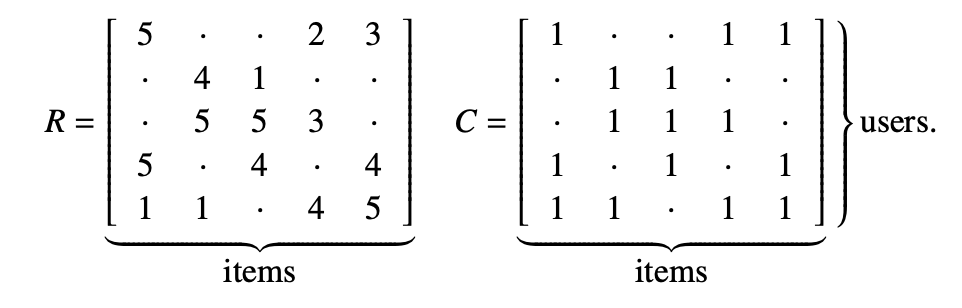
\includegraphics[width=0.75\linewidth]{images/R_C.png}
    \caption{User-item interaction matrices (R=ratings, C=interactions)}
    \label{fig:rc}
\end{figure}

Our next question is, “How to extract the necessary features from the user-item interactions without knowing or observing them?”, which is essentially the goal of \textbf{Matrix Factorization}, which looks for the underlying low-dimensional structure that explains these observations. 

Figure \ref{fig:mf} shows the goal of approximating a partially observed matrix in terms of lower-dimensional factors. We assume that $R_{|U|\times|I|}$ can be expressed as the matrix product of a tall matrix $\gamma_U$ and a fat matrix $\gamma_I$, such that the individual entries in $R_{u,i}$ can be estimated by taking the dot product of the corresponding row of $\gamma_U$ and the column of $\gamma_I$., i.e. $R_{u,i} = \gamma_U \cdot \gamma_I$. Here, $\gamma_U$ and $\gamma_U$ are vectors that represent the latent factors describing the user $u$ and item $i$ respectively. We can think of $\gamma_U$ as the features that represent the preferences of the user $u$ and $\gamma_I$ as the features that describe the item $i$. Hence, $u$ will have a high interaction with $i$ if they have compatible features.
Figure \ref{fig:ui_vectors} depicts such vectors.

\begin{figure}
    \centering
    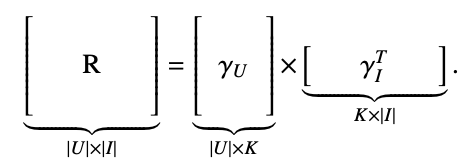
\includegraphics[width=0.75\linewidth]{images/SVD.png}
    \caption{Factorization of the user-item interactions matrix R}
    \label{fig:mf}
\end{figure}

\begin{figure}[h]
    \centering
    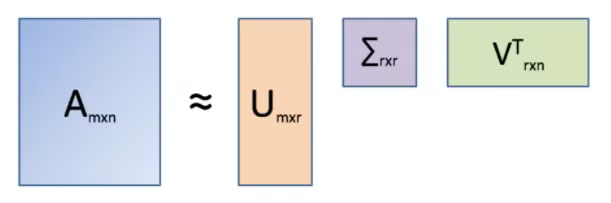
\includegraphics[width=0.75\linewidth]{images/image2.png}
    \caption{Singular Value Decomposition}
    \label{fig:svd}
\end{figure}

\begin{figure}[h]
\centering
\begin{minipage}{.3\textwidth}
  \centering
  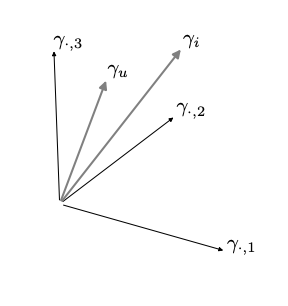
\includegraphics[width=.9\linewidth]{DSC210_Project_Report/images/ui_vectors.png}
  \caption{Representation of user $u$ and item $i$ in latent factor model}
  \label{fig:ui_vectors}
\end{minipage}%
\begin{minipage}{.7\textwidth}
  \centering
  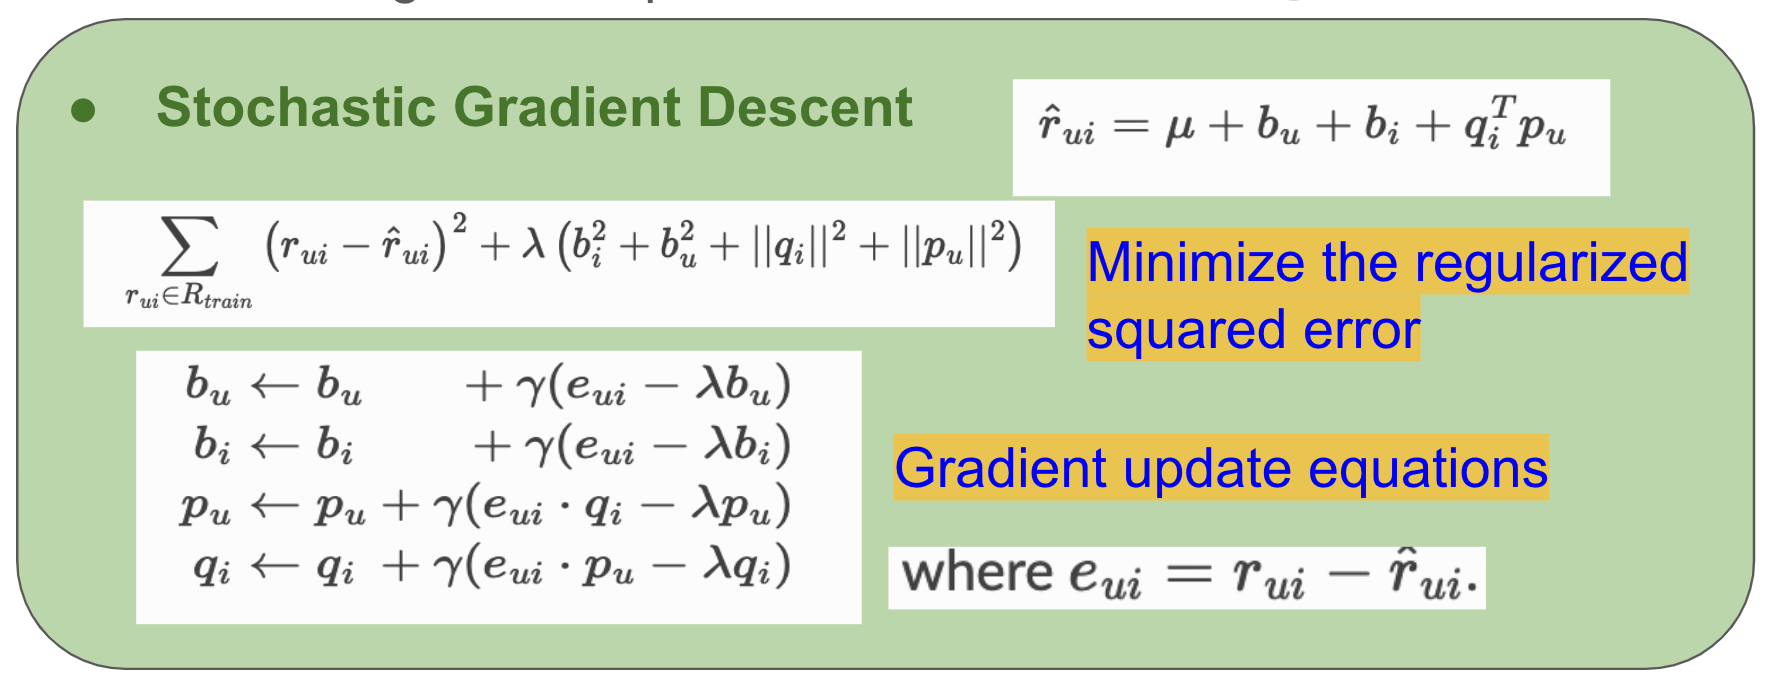
\includegraphics[width=.9\linewidth]{DSC210_Project_Report/images/sgd.png}
  \caption{SGD}
  \label{fig:sgd}
\end{minipage}
\end{figure}

This process of matrix factorization is strongly related to the SVD technique. The SVD of a real-valued matrix $A$ is given by $A=U \Sigma V^T$, where $U$ and $V$ are left and right singular values of $A$ (eigenvectors of $AA^T$ and $A^T A$), and $\Sigma$ is a diagonal matrix of eigenvectors of $AA^T$ (or $A^T A$). Critically, the best low-rank approximation of $A$ (say rank=r, in terms of the mean squared error) is found by taking the top r eigenvectors/eigenvalues in $U$, $\Sigma$ and $V$ (Eckart- Young theorem). If $u_i$s are the columns of $U$, $\sigma_i$s are the diagonal values in $\Sigma$, and $v_i^T$s are the rows of $V^T$, then

$A_r = \sum_{i=1}^{r} \sigma_i u_i v_i^T \quad , \sigma_1 \ge \sigma_2 \ge .. \ge 0$

Since it is impractical to compute SVD directly on large matrices, Alternating Least Squares \cite{als} or Stochastic Gradient Descent \cite{matfact} is often used for the computation.

The prediction $\hat{r}_{ui}$ is set as $\hat{r}_{ui} = \mu + b_u + b_i + q_i^Tp_u$.
If user $u$ is unknown, then the bias $b_u$ and the factors $p_u$ are assumed to be zero. The same applies for item $i$ with $b_i$ and $q_i$.
To estimate all the unknown, we minimize the following regularized squared error using Stochastic Gradient Descent:
$\sum_{r_{ui} \in R_{train}} (r_{ui} - \hat{r}_{ui})^2 + \lambda (b_i^2 + b_u^2 + ||q_i||^2 + ||p_u||^2)$ (which includes regularization).
% \newpage
\subsection{Approach description}

A Bayesian Personalized Ranking (BPR) approach will provide a scalable method addressing to the limitations observed in SVD-based recommender systems. Bayesian theory and the Bayesian statistics form the foundation of BPR. Further, \textbf{Bayes’ Rule} provides the mathematical rule for inverting conditional probability distributions, allowing us to measure the likelihood that a particular event will occur. Inverse probability transforms a prior distribution of a parameter, combined with the conditional distribution of the data, into the posterior distribution of that parameter\cite{SCHWEDER200115031}. The rule depends on knowing previous events that have taken place in order to form the probability.
%\begin{center}
%    \textit{Conditional probability where B is a known variable:}\\
%    $P(A|B)=\frac{P(A\cap B)}{P(B)}$
%\end{center}
\begin{figure}[ht]
    \centering
    $P(A|B)=\frac{P(A\cap B)}{P(B)}$
    \caption{Conditional probability where B is a known variable}
    \label{fig:conditional-prob}
\end{figure}

In the context of recommendation systems, we predict what item a user is most likely going to have interest in, with our known variable depending on previous events, or observed interactions such as clicks or past purchases. When limited information is available for our known variable, we can invert the conditional probability using Bayes’ Theorem\cite{bayes}. We can apply the Theorem by allowing \(A = Items\) and \(B = Clicks\). 
%\begin{center}
%    \textit{Bayes' Theorem:}\\
%    $P(A|B)=\frac{P(A)P(B|A)}{P(B)}$
%\end{center}

\begin{figure}[ht]
    \centering
    $P(A|B)=\frac{P(A)P(B|A)}{P(B)}$
    \caption{Bayes' Theorem}
    \label{fig:Bayes-theorem}
\end{figure}

We can further apply Bayes' theorem for optimization by introducing the latent factors of user \(u\) and a parameter vector, \(\Theta\), of our matrix factorization: \(p(\Theta | >_u) \propto p(>_u | \Theta)p(\Theta) \) \cite{bpr-arix}.
Here, our posterior probability \(p(\Theta | >_u)\) represents the update in parameters \(\Theta\) following our observation in the user latent factor data \(>_u\). The posterior probability is proportional to the likelihood of observing the data and the parameters \(p(>_u | \Theta)\) multiplied by the prior probability of \(p(\Theta)\). We aim to maximize the posterior probability of the equation. In BPR, this method allows us to integrate prior knowledge and update it with observed data to improve our predictions. \\~\\
The Bayes’ Theorem is expanded upon in BPR to measure the pairwise interactions between a user and an item in order to identify if a user \(u\), has a preference of item \(i\) over item \(j\). We can assume each user has independent preferences and that each item pair of \(i\) and \(j\) will have a unique relationship with each user introducing the use of the preference probability and the logistic function\cite{bpr-arix}:
%\begin{center}
%    \(p(i>_u j|\Theta):= \sigma(\hat x_{uij}(\Theta)), \textit{Where } \sigma(x) := \frac{1}{1+e^{-x}} \) \\
%\end{center}

\begin{figure}[ht]
    \centering
    $p(i>_u j|\Theta):= \sigma(\hat x_{uij}(\Theta)), \textit{Where } \sigma(x) := \frac{1}{1+e^{-x}} $
    \caption{Logistic Function}
    \label{fig:logistic-func}
\end{figure}

Here, $\hat x_{uij}$ is decomposed as $\hat x_{ui} - \hat x_{uj}$. Now that we have defined our pairwise preference and are able to acquire an interaction score using our probability function we can begin to formulate a loss function to maximize the users preference and minimize the difference between the prediction of a user preferring item \(i\) over \(j\) or vice-versa. Differentiable, or logistic loss \cite{bpr-arix} is defined by \(ln \theta(x)\), for our tuple \(u, i, j\) in dataset \(D\) where $\lambda_{\Theta}$ is the regularization:
%\vspace{-1cm}
\begin{center}
    \[
    Loss = - \sum_{(u, i, j) \in D} ln(p(i>_{u} j|\Theta)) p(\Theta) 
    = - (\sum_{(u, i, j) \in D} ln (\sigma(\hat x_{uij}) - \lambda_{\Theta} ||\Theta||^2)
    \]
\end{center}


Analogous to AUC (Area Under ROC Curve), this can also be formulated as 
\[\text{AUC}(u) := \frac{1}{|I_u^+| |I \setminus I_u^+|} \sum_{i \in I_u^+} \sum_{j \in |I \setminus I_u^+|} \delta(\hat{x}_{uij} > 0)\]
Plus (+) indicates that a user prefers item $i$ over item $j$; minus (–) indicates that he prefers $j$ over $i$. The AUC uses the non-differentiable loss
\[
\delta(x > 0) \text{ which is identical to the Heaviside function:}
\delta(x > 0) = H(x) := \begin{cases}
1, & x > 0 \\
0, & \text{else}
\end{cases}
\]

In our implementation we leverage the \textit{implicit} package from python and import \textit{bpr.BayesianRankingPersonalization} which utilizes the above logistic loss function. 
% \textit{Implicit} also implements \textbf{Alternating Least Squares (ALS)} as an optimization algorithm for BPR. With ALS, the optimization process scales linearly with the size of the data\cite{als} providing a well suited method of scaling BPR across large datasets. ALS can effectively minimize the loss function of our pairwise preferences by alternating between fixing the users latent vectors and optimizing the items until convergence is achieved. 

\subsection{SOTA approach description}

A transformer model is a type of neural network that learns context and meaning by capturing relationships in sequential data. It was first introduced in 2017 by a team from Google \cite{transformer}. The key innovation of the transformer architecture is the self-attention mechanism, which allows the model to weigh the importance of different elements in a sequence, regardless of their position. This ability to consider all parts of a sequence simultaneously, rather than processing it step-by-step, enables transformers to efficiently capture complex dependencies and long-range relationships. Since its introduction, transformers have been regarded as "foundational models" in AI and are widely considered to be driving a paradigm shift in fields such as natural language processing (NLP), computer vision, and beyond.

BERT4Rec \cite{sun2019bert4rec} is a cutting-edge sequential recommendation model that applies the transformer architecture, specifically leveraging the BERT (Bidirectional Encoder Representations from Transformers) framework, to the task of personalized recommendations. Unlike traditional collaborative filtering approaches that rely on matrix factorization or explicit neighborhood modeling, BERT4Rec is designed to capture sequential patterns in user behavior. It models user-item interactions as a sequence prediction task, learning rich representations of user preferences over time. The self-attention mechanism of BERT enables BERT4Rec to consider the importance of each item in a user's history, providing a more holistic understanding of user preferences.

One of the key innovations of BERT4Rec is its bidirectional training paradigm. Traditional sequential recommendation models, such as RNN-based or auto-regressive methods, typically predict the next item based on past interactions in a unidirectional manner. BERT4Rec, on the other hand, allows the model to look at both past and future interactions simultaneously by masking items during training. This approach encourages the model to learn from both the left and right contexts in a sequence, which results in more accurate item recommendations.

In the context of the Amazon dataset, where users interact with a wide variety of products over time, BERT4Rec is particularly effective. The model can handle the complexities of real-world recommendation scenarios, such as dealing with sparse data, long user histories, and varying interaction patterns. It can also incorporate implicit feedback (like clicks or views) and explicit signals (such as ratings), making it highly adaptable for a large and diverse dataset like Amazon’s, where user behavior is highly varied.

Additionally, BERT4Rec's transformer architecture enables it to scale well to large datasets, such as Amazon’s, by taking advantage of parallelism during training. This scalability, combined with the model's ability to capture long-term dependencies in user interactions, makes BERT4Rec a powerful tool for providing highly personalized and relevant item recommendations in e-commerce platforms. By leveraging the contextual information embedded in user sequences, BERT4Rec has set a new benchmark in the field of sequential recommendation systems.

\begin{figure}
    \centering
    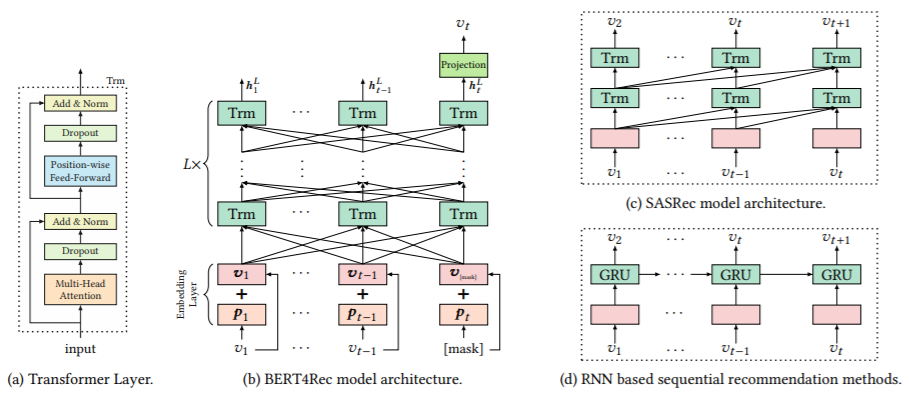
\includegraphics[width=1.1\linewidth]{DSC210_Project_Report/images/bert4rec.png}
    \caption{Bert4Rec architecture}
    \label{fig:mf}
\end{figure}
While BPR and SVD remain robust baselines for personalized ranking and collaborative filtering in static recommendation settings, self-attentive sequential models represent a significant advancement in modeling user preferences over time. By explicitly capturing intricate patterns in user behavior, these models excel in sequential tasks, offering superior personalization and predictive performance. This makes self-attentive sequential models indispensable in modern recommendation system design, where dynamic user behavior and context are critical.

% \begin{figure}[h]
% \centering
% \begin{minipage}{.5\textwidth}
%   \centering
%   \includegraphics[width=.9\linewidth]{image5.png}
% \end{minipage}%
% \begin{minipage}{.5\textwidth}
%   \centering
%   \includegraphics[width=.9\linewidth]{image6.png}
% \end{minipage}
% \end{figure}


\section{Experiments}
\subsection{Setup and logistics}
\begin{itemize}
    \item We use Python as the programming language for this project. We will use Google Colab to develop the code and use GitHub for version control.
    \item We load the data from the HuggingFace dataset repository, and use several data-science libraries. We will use functions and APIs from NumPy, Pandas, Matplotlib, Surprise \cite{surprise}, Implicit \footnote{https://github.com/benfred/implicit}, PyTorch, and Transformers.
    
    % WordCloud, and Umap are used for graphs and visualization. 
\end{itemize}
SVD hyperparameters:
\begin{itemize}
    \item \texttt{n\_factors}: The number of factors. Default is 100.
    \item \texttt{n\_epochs}: The number of iteration of the SGD procedure. Default is 20.
    \item \texttt{biased}: Whether to use baselines (or biases). See note above. Default is True.
    \item \texttt{init\_mean}: The mean of the normal distribution for factor vectors initialization. Default is 0.
    \item \texttt{init\_std\_dev}: The standard deviation of the normal distribution for factor vectors initialization. Default is 0.1.
    \item \texttt{lr\_all}: The learning rate for all parameters. Default is 0.005.
    \item \texttt{reg\_all}: The regularization term for all parameters. Default is 0.02.
    \item \texttt{lr\_bu}: The learning rate for $b_u$. Takes precedence over \texttt{lr\_all} if set. Default is None.
    \item \texttt{lr\_bi}: The learning rate for $b_i$. Takes precedence over \texttt{lr\_all} if set. Default is None.
    \item \texttt{lr\_pu}: The learning rate for $p_u$. Takes precedence over \texttt{lr\_all} if set. Default is None.
    \item \texttt{lr\_qi}: The learning rate for $q_i$. Takes precedence over \texttt{lr\_all} if set. Default is None.
    \item \texttt{reg\_bu}: The regularization term for $b_u$. Takes precedence over \texttt{reg\_all} if set. Default is None.
    \item \texttt{reg\_bi}: The regularization term for $b_i$. Takes precedence over \texttt{reg\_all} if set. Default is None.
    \item \texttt{reg\_pu}: The regularization term for $p_u$. Takes precedence over \texttt{reg\_all} if set. Default is None.
    \item \texttt{reg\_qi}: The regularization term for $q_i$. Takes precedence over \texttt{reg\_all} if set. Default is None.
    \item \texttt{random\_state}: Determines the RNG that will be used for initialization. If int, \texttt{random\_state} will be used as a seed for a new RNG. This is useful to get the same initialization over multiple calls to \texttt{fit()}. If RandomState instance, this same instance is used as RNG. If None, the current RNG from numpy is used. Default is None.
    \item \texttt{verbose}: If True, prints the current epoch. Default is False.
\end{itemize}

BPR hyperparameters (with =defaults):
\begin{itemize}
    \item \texttt{factors=100}: Number of latent factors
    \item \texttt{learning\_rate=0.01}: Learning rate for training
    \item \texttt{regularization=0.01}: Regularization parameter
    \item \texttt{iterations=100}: Number of training iterations
    \item \texttt{verify\_negative\_samples=True}: Whether to verify negative samples
    \item \texttt{random\_state=None}: Random seed for initialization
\end{itemize}

SOTA hyperparameters: 
\begin{itemize}
    \item \texttt{hidden\_size (int)}: The number of features in the hidden state. It is also the initial embedding size of items. Defaults to \texttt{64}.
    
    \item \texttt{inner\_size (int)}: The inner hidden size in the feed-forward layer. Defaults to \texttt{256}.
    
    \item \texttt{n\_layers (int)}: The number of transformer layers in the transformer encoder. Defaults to \texttt{2}.
    
    \item \texttt{n\_heads (int)}: The number of attention heads for the multi-head attention layer. Defaults to \texttt{2}.
    
    \item \texttt{hidden\_dropout\_prob (float)}: The probability of an element being zeroed. Defaults to \texttt{0.5}.
    
    \item \texttt{attn\_dropout\_prob (float)}: The probability of an attention score being zeroed. Defaults to \texttt{0.5}.
    
    \item \texttt{hidden\_act (str)}: The activation function in the feed-forward layer. Defaults to \texttt{gelu}. Range: \texttt{['gelu', 'relu', 'swish', 'tanh', 'sigmoid']}.
    
    \item \texttt{layer\_norm\_eps (float)}: A value added to the denominator for numerical stability. Defaults to \texttt{1e-12}.
    
    \item \texttt{loss\_type (str)}: The type of loss function. If it is set to \texttt{CE}, the training task is regarded as a multi-classification task, and the target item is the ground truth. In this way, negative sampling is not needed. If it is set to \texttt{BPR}, the training task will be optimized in a pair-wise way, which maximizes the difference between the positive item and the negative one. In this way, negative sampling is necessary, such as setting \texttt{--train\_neg\_sample\_args="\{'distribution': 'uniform', 'sample\_num': 1\}"}. Defaults to \texttt{CE}. Range in \texttt{['BPR', 'CE']}.
\end{itemize}

\subsection{Dataset and programming}

Let us see the implementation in code:

\textbf{Preprocessing} Joel could you please add this (importing packages, loading the dataset etc.)

\textbf{Singular Value Decomposition}: We leverage the surprise library \footnote{https://surprise.readthedocs.io/en/stable/} for this task. It uses Stochastic Gradient Descent as a gradient-based approach to solve the formulated predicted rating $\hat{r}_{ui}$ as explained earlier in \ref{fig:sgd}.
\begin{lstlisting}[language=Python]
# Number of latent factors
k = 5

# Initialize the Single Value Decomposition model for collaborative filtering
svd = SVD(n_factors = k, verbose = True)

#Split the data into training and test sets. Only use 25% of the data for speed.
trainset, testset = train_test_split(surprise_data, test_size=.25, random_state=random_state)

# Fit the model to the training set
svd.fit(trainset)

# Assign predictions to the test set of the trained model
predictions = svd.test(testset)

# root mean squared error
accuracy.rmse(predictions, verbose=True)

# A sample Prediction contains the user id (uid), item id(iid), actual rating (r_ui), estimated rating (est), and additional details (details).
(predictions[0])

def get_top_n(predictions, n=3):
    """Return the top-N recommendation for each user from a set of predictions.

    Args:
        predictions(list of Prediction objects): The list of predictions, as
            returned by the test method of an algorithm.
        n(int): The number of recommendation to output for each user. Default
            is 10.

    Returns:
    A dict where keys are user (raw) ids and values are lists of tuples:
        [(raw item id, rating estimation), ...] of size n.
    """

    # First map the predictions to each user.
    top_n = defaultdict(list)
    for uid, iid, true_r, est, _ in predictions:
        top_n[uid].append((iid, est))

    # Then sort the predictions for each user and retrieve the k highest ones.
    for uid, user_ratings in top_n.items():
        user_ratings.sort(key=lambda x: x[1], reverse=True)
        top_n[uid] = user_ratings[:n]

    return top_n

top_n = get_top_n(predictions, n=3)
# Print the recommended items for the first user
uid0, iids = None, None
for uid, user_ratings in top_n.items():
    uid0 = uid
    iids = [iid for (iid, _) in user_ratings]
print(f"User id that we inspect: {uid0}")
# Check what the user has reviewed
user0_reviews = DS.from_pandas(df).filter(lambda row: row["user_id"] == uid0)
user0_reviewed_items = user0_reviews["parent_asin"]
user0_reviewd_items_images = dataset_items.filter(lambda row: row["parent_asin"] in user0_reviewed_items)

# takes the dataset and fetches 2 large sized images of each item using its url
def show_images(dataset):
    image_urls = []
    # URL of the image
    for img in dataset["full"]["images"]:
        for large_image in img["large"][:2]: # show 2 images of each item that is recommended
            image_urls.append(large_image)

    for url in image_urls:
        # Fetch and display the image
        response = requests.get(url)
        img = Image.open(BytesIO(response.content))
        # Display the image inline
        plt.imshow(img)
        plt.axis('off')  # Turn off axis labels
        plt.show()

show_images(user0_reviewd_items_images)

# Check what the model recommends for the user
uid0_images = []
filtered_dataset = dataset_items.filter(lambda row: row["parent_asin"] in iids)

filtered_dataset["full"].to_pandas().head()
show_images(filtered_dataset)

def precision_recall_at_k(predictions, k=10, threshold=3.5):
    """Return precision and recall at k metrics for each user"""

    # First map the predictions to each user.
    user_est_true = defaultdict(list)
    for uid, _, true_r, est, _ in predictions:
        user_est_true[uid].append((est, true_r))

    precisions = dict()
    recalls = dict()
    for uid, user_ratings in user_est_true.items():

        # Sort user ratings by estimated value
        user_ratings.sort(key=lambda x: x[0], reverse=True)

        # Number of relevant items
        n_rel = sum((true_r >= threshold) for (_, true_r) in user_ratings)

        # Number of recommended items in top k
        n_rec_k = sum((est >= threshold) for (est, _) in user_ratings[:k])

        # Number of relevant and recommended items in top k
        n_rel_and_rec_k = sum(
            ((true_r >= threshold) and (est >= threshold))
            for (est, true_r) in user_ratings[:k]
        )

        # Precision@K: Proportion of recommended items that are relevant
        # When n_rec_k is 0, Precision is undefined. We here set it to 0.

        precisions[uid] = n_rel_and_rec_k / n_rec_k if n_rec_k != 0 else 0

        # Recall@K: Proportion of relevant items that are recommended
        # When n_rel is 0, Recall is undefined. We here set it to 0.

        recalls[uid] = n_rel_and_rec_k / n_rel if n_rel != 0 else 0

    return precisions, recalls

precisions, recalls = precision_recall_at_k(predictions, k=3, threshold=4)

# Take the average over all values
precision = np.mean(np.array([prec for prec in precisions.values()]))
recall = np.mean(np.array([rec for rec in recalls.values()]))
print(f"Precision={precision}, recall={recall}")
\end{lstlisting}

\textbf{Bayesian Personalized Ranking}: We leverage the implicit \footnote{https://github.com/benfred/implicit} library for this task.
\begin{lstlisting}[language=Python ]
# Create a new BPR dataframe
df_bpr = pd.DataFrame(dataset['full'][:len(dataset['full']) // 10]).sample(frac=.5, random_state=random_state)
random_state = 33

# Store the number of time each user and each item is associated with a review
user_id_counts, parent_id_counts = defaultdict(int), defaultdict(int)
for idx, row in tqdm(df.iterrows()):
    user_id, item_id, parent_item_id = row["user_id"], row["asin"], row["parent_asin"]
    user_id_counts[user_id] += 1
    parent_id_counts[parent_item_id] += 1

df = df_bpr
# Grid search parameters to find a suitable threshold for the number of times a user and an item are associated with a review. This helps deal with extremely sparse data and provides more interpretable recommendations.
threshold_users_list = [10, 20, 30, 35, 40]
threshold_parents_list = [25, 50, 75, 100, 125, 150]

bpr_precisions = []
bpr_aucs = []
bpr_ndcgs = []
threshold_pairs = []
models = []

for threshold_users in threshold_users_list:
    for threshold_parents in threshold_parents_list:
        # userIDs is a map from user_id to index
        # itemIDS is a map from item_id to index
        # indexToUser is a map from the index to the user ID
        # indexToItem is a map from the index to the item ID
        # asinToParentAsin is a map from asin to parent asin (item ID of all variants)
        # Assign our variables with empty dictionaries
        userIDs, itemIDs, indexToUser, indexToItem, parentIDs, indexToParent, asinToParentAsin = {}, {}, {}, {}, {}, {}, {}

        # Iterate over the dataframe rows
        for idx, row in tqdm(df.iterrows()):
            # Assign our variables to associations in our dataset
            user_id, item_id, parent_item_id = row["user_id"], row["asin"], row["parent_asin"]

            # Check if user_id is already in the dictionary, if not then assign it with a unique index
            if user_id not in userIDs and user_id_counts[user_id] >= threshold_users:
                userIDs[user_id] = len(userIDs)
                indexToUser[userIDs[user_id]] = user_id

            # Check item_ids inside the dictionary
            if item_id not in itemIDs:
                # Assign unique index to the item_id
                itemIDs[item_id] = len(itemIDs)
                # Map the index to the item
                indexToItem[itemIDs[item_id]] = item_id
                # Associate the item_id to the parent item id
                asinToParentAsin[item_id] = parent_item_id

            # Add the parent to the set of unique parentIDs
            if parent_item_id not in parentIDs and parent_id_counts[parent_item_id] >= threshold_parents:
                parentIDs[parent_item_id] = len(parentIDs)
                indexToParent[parentIDs[parent_item_id]] = parent_item_id


        # Get the lengths to print the totals
        nUsers, nItems, nParents = len(userIDs), len(itemIDs), len(parentIDs)
        print(f"For threshold_users = {threshold_users}, threshold_items = {threshold_parents}, there are a total of {nUsers} users and {nParents} products with a total of {nItems} items including all variants.")

        # Initialized after extracting the number of users and items
        Xui = scipy.sparse.lil_matrix((nUsers, nParents))

        # Iterate over each row in the dataframe
        for ifx, row in tqdm(df.iterrows()):
            user_id, item_id = row["user_id"], row["parent_asin"]
            if user_id_counts[user_id] >= threshold_users and parent_id_counts[item_id] >= threshold_parents:
              #Only storing positive feedback instances
              Xui[userIDs[user_id],parentIDs[item_id]] = 1

        # Convert matrix to a compressed sparse row
        Xui_csr = scipy.sparse.csr_matrix(Xui)

#         print(Xui_csr)
        print(f"Sparsity of the matrix = {(1 - (Xui_csr.nnz/(Xui_csr.shape[0]*Xui_csr.shape[1]))):.6f}%")

        Xui_train, Xui_test = leave_k_out_split(Xui_csr, K=1, random_state=random_state)

        # Hyperparameter of latent factors
        k = 5
        # Initialze the BPR model with the hyperparameters
        model = bpr.BayesianPersonalizedRanking(factors = k, random_state=random_state, iterations=100, regularization=0.01)
        # Fit the BPR model to the training set
        model.fit(Xui_train)
        bpr_precision = precision_at_k(model, Xui_train, Xui_test, 10, True)
        bpr_auc = AUC_at_k(model, Xui_train, Xui_test, 10, True)
        bpr_ndcg = ndcg_at_k(model, Xui_train, Xui_test, 10, True)
        threshold_pairs.append((threshold_users, threshold_parents))
        models.append(model)
    #     print(f"Precision={bpr_precision}, AUC={bpr_auc}, NDCG={bpr_ndcg}")
        bpr_precisions.append(bpr_precision)
        bpr_aucs.append(bpr_auc)
        bpr_ndcgs.append(bpr_ndcg)

# Get the maximum respective metric
max_precision_index = bpr_precisions.index(max(bpr_precisions))
max_auc_index = bpr_aucs.index(max(bpr_aucs))
max_ndcg_index = bpr_ndcgs.index(max(bpr_ndcgs))

# Plot the precision@K
plt.figure(figsize=(8, 5))
plt.plot(list(range(1, len(threshold_users_list)*len(threshold_parents_list) + 1)), bpr_precisions, marker='o', linestyle='-', color='b', label='y vs x')
plt.xlabel('threshold pairs')
plt.ylabel('precision@K')
plt.title('BPR precision@K')
plt.legend()
plt.grid(True)
plt.show()
print(f"The max precision@K = {bpr_precisions[max_precision_index]} for threshold_users = {threshold_pairs[max_precision_index][0]} and threshold_parents = {threshold_pairs[max_precision_index][1]}")

# Plot the AUC@K
plt.figure(figsize=(8, 5))
plt.plot(list(range(1, len(threshold_users_list)*len(threshold_parents_list) + 1)), bpr_aucs, marker='o', linestyle='-', color='b', label='y vs x')
plt.xlabel('threshold pairs')
plt.ylabel('auc@K')
plt.title('BPR auc@K')
plt.legend()
plt.grid(True)
plt.show()
print(f"The max auc@K = {bpr_aucs[max_auc_index]} for threshold_users = {threshold_pairs[max_auc_index][0]} and threshold_parents = {threshold_pairs[max_auc_index][1]}")

#Plot the NDCG@K
plt.figure(figsize=(8, 5))
plt.plot(list(range(1, len(threshold_users_list)*len(threshold_parents_list) + 1)), bpr_ndcgs, marker='o', linestyle='-', color='b', label='y vs x')
plt.xlabel('threshold pairs')
plt.ylabel('ndcg@K')
plt.title('BPR ndcg@K')
plt.legend()
plt.grid(True)
plt.show()
print(f"The max ndcg@K = {bpr_ndcgs[max_ndcg_index]} for threshold_users = {threshold_pairs[max_ndcg_index][0]} and threshold_parents = {threshold_pairs[max_ndcg_index][1]}")

# Load the best AUC model to visualize recommendations
model = models[max_auc_index] # let us use the best AUC model

itemFactors = model.item_factors
userFactors = model.user_factors

uid0index = 2
recommended = model.recommend(uid0index, Xui_test[uid0index]) # Top k Recommendations for the user
print(recommended)
print(f"Inspecting items for user {uid0}")
# Create an empty list for the recommended items
recommended_items = []

# Loop over each recommended ID
for recommendedId in recommended[0]:

    # Search for rows where the parent asin matches
    row = df_items[df_items["parent_asin"] == indexToParent[recommendedId]]

    # Append the rows to the recommended items list
    recommended_items.append(row)

# Concatonate the dataframes into a single frame
x = pd.concat(recommended_items, ignore_index=True)
print(len(x))

# Show the concatonated dataframe
x
# show the images of the recommended items
def show_images(dataset):
    image_urls = []
    # URL of the image
    for img in dataset["images"]:
        for large_image in img["large"][:1]: # show 2 images of each item that is recommended
            image_urls.append(large_image)

    for url in image_urls:
        # Fetch and display the image
        response = requests.get(url)
        img = Image.open(BytesIO(response.content))
        # Display the image inline
        plt.imshow(img)
        plt.axis('off')  # Turn off axis labels
        plt.show()

show_images(x)

indexOfRelatedItem = 4
related = model.similar_items(indexOfRelatedItem) # Top 10 Highly similar to the 5th item (using cosine similarity)
print(related) # shows the index of the similar item and the similarity score (sorted from best to least)
# What is the 5th item?
x = df_items[df_items["parent_asin"] == indexToParent[indexOfRelatedItem]]
print(x)
show_images(x)

# Create an empty list for the related items
related_items = []

# Loop over the related ID's
for relatedId in related[0]:
    # Find the parent ASIN coresponding to the related item ID
    parent_asin = indexToParent[relatedId]

    # Find rows where the parent asin matches
    row = df_items[df_items["parent_asin"] == parent_asin]

    # Append the row items to the related items list
    related_items.append(row)

# Concatonate the dataframes into a single dataframe
x = pd.concat(related_items, ignore_index=True)
print(len(x))

# Print the concatonated dataframe
x
\end{lstlisting} 

\subsection{Results}

For SVD, we can generate much lower dimensional latent factor representations of users and items that can approximate the original matrix as shown by the reconstruction.
We calculate the precision@K, recall@K and f1@K to be x, y, and z respectively.

However, this assumes fully observed data, so as discussed, previously, we want to move to the BPR model.
For BPR, we calculate the precision@K, AUC@K, NDCG@K shown in Fig \ref{fig:bpr_precision}, Fig \ref{fig:bpr_auc} and Fig \ref{fig:bpr_ndcg} respectively, with K=10. 

\begin{figure}[ht]
    \centering
    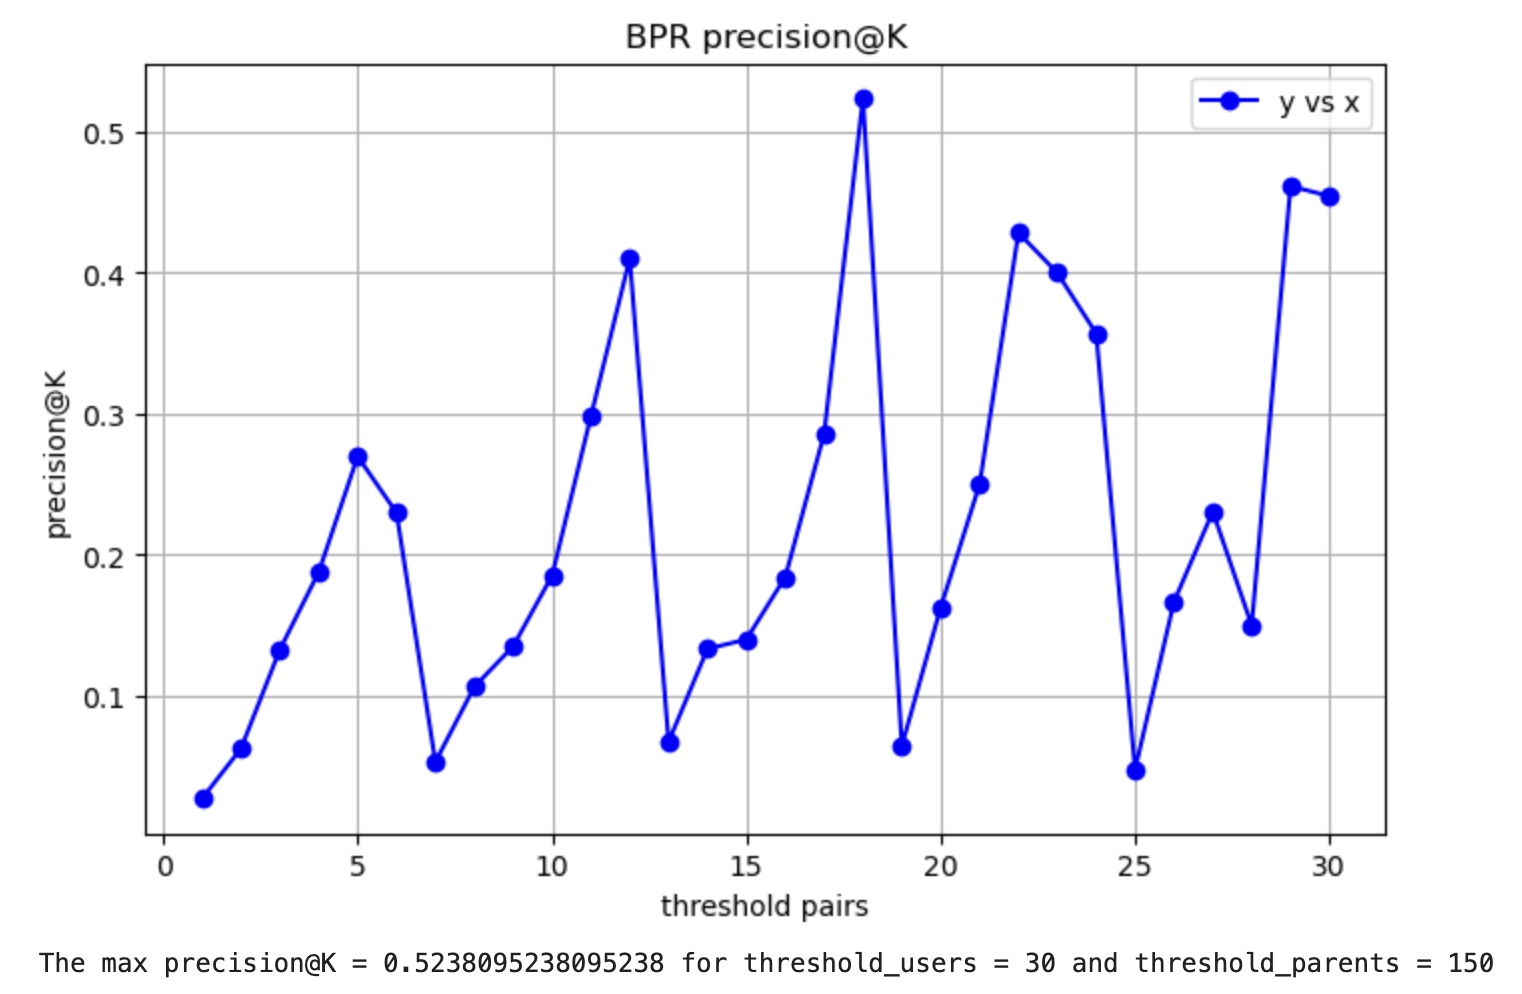
\includegraphics[width=0.75\linewidth]{DSC210_Project_Report/images/bpr_plot_precision.png}
    \caption{Precision vs threshold pairs}
    \label{fig:bpr_precision}
\end{figure}
\begin{figure}
    \centering
    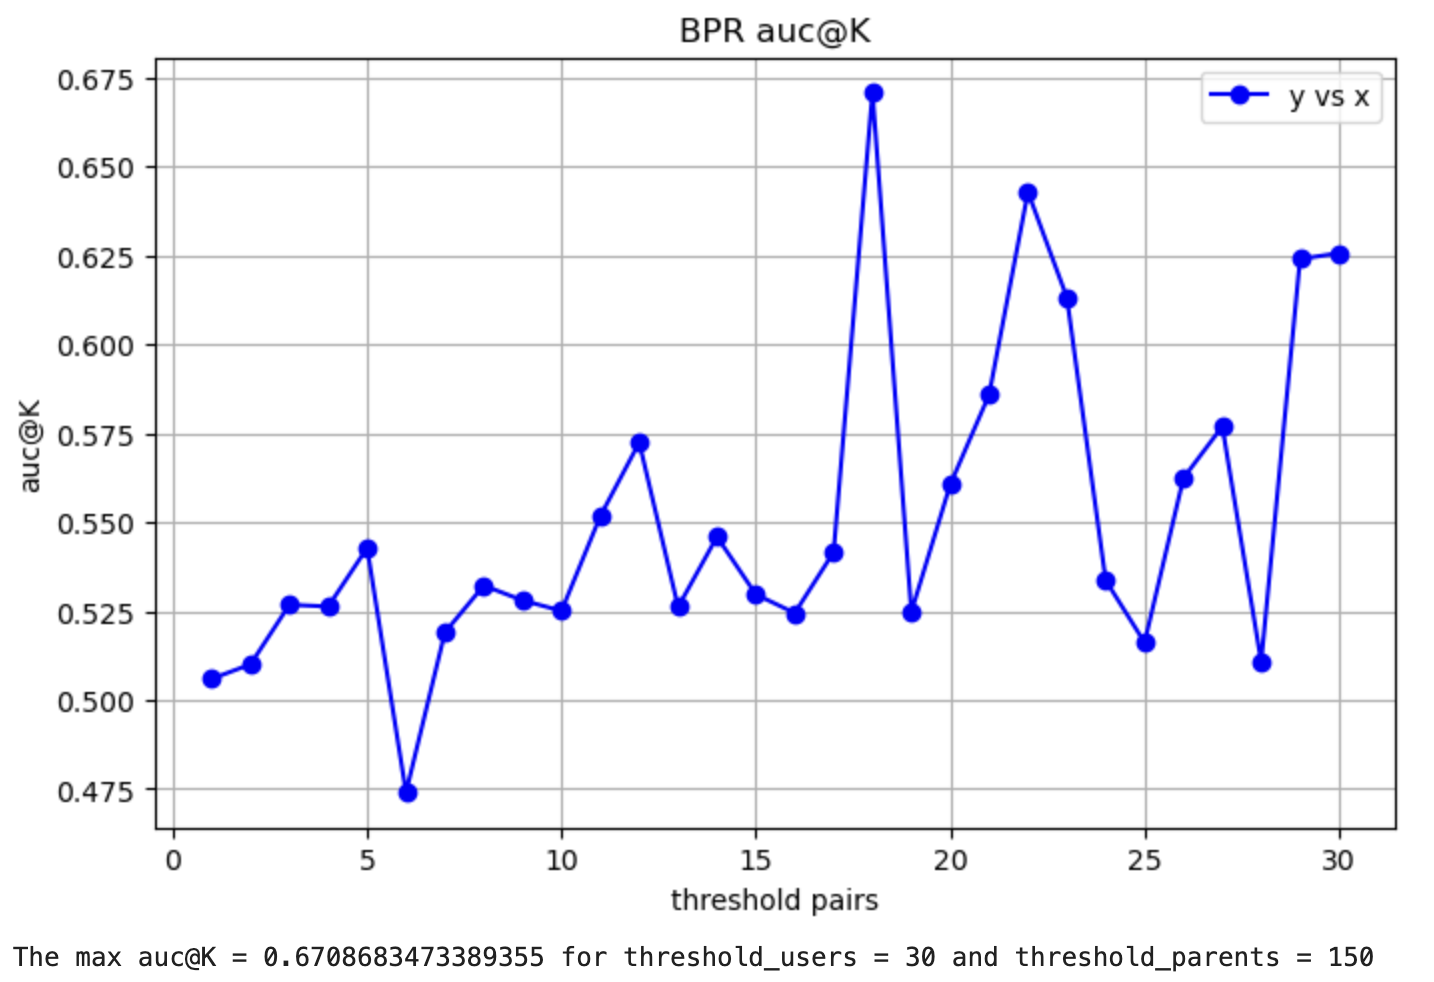
\includegraphics[width=0.75\linewidth]{DSC210_Project_Report/images/bpr_plot_auc.png}
    \caption{AUC vs threshold pairs}
    \label{fig:bpr_auc}
\end{figure}
\begin{figure}
    \centering
    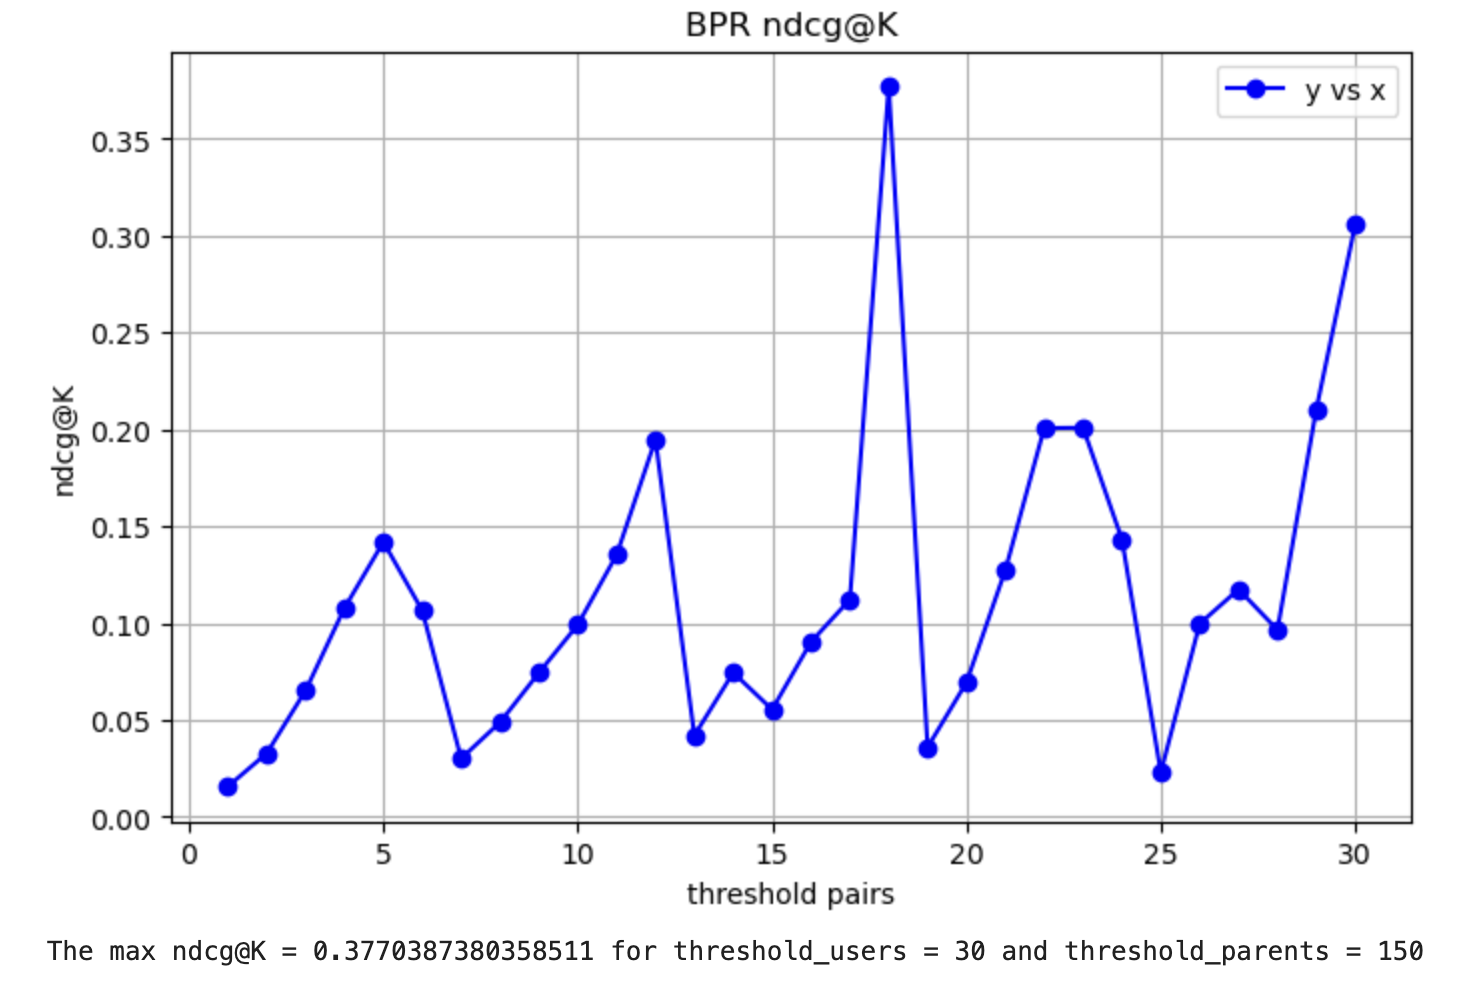
\includegraphics[width=0.75\linewidth]{DSC210_Project_Report/images/bpr_plot_ndcg.png}
    \caption{NDCG vs threshold pairs}
    \label{fig:bpr_ndcg}
\end{figure}

Although the matrix remains highly sparse (96\%-99\%), we see that there is improved reliability of the recommendations when we deal with frequent users and popular items. The trend of popular items is also observed among all 3 metrics. For every user threshold, we tend to see better scores for the more popular items (associated with more reviews). This aligns with our intuition that recommended items will tend to also be popular among users.

We visualize the recommended items for the user who is associated with guitar reviews in \ref{fig:bpr_recommendations}, and we see accessories for guitar being recommended.
\begin{figure}[h]
\centering
\begin{minipage}{.3\textwidth}
  \centering
  
\includegraphics[width=.9\linewidth]{DSC210_Project_Report/images/recommendation1.png}
\end{minipage}%
\begin{minipage}{.3\textwidth}
  \centering
  
\includegraphics[width=.9\linewidth]{DSC210_Project_Report/images/recommendation2.png}
\end{minipage}
\begin{minipage}{.3\textwidth}
  \centering
  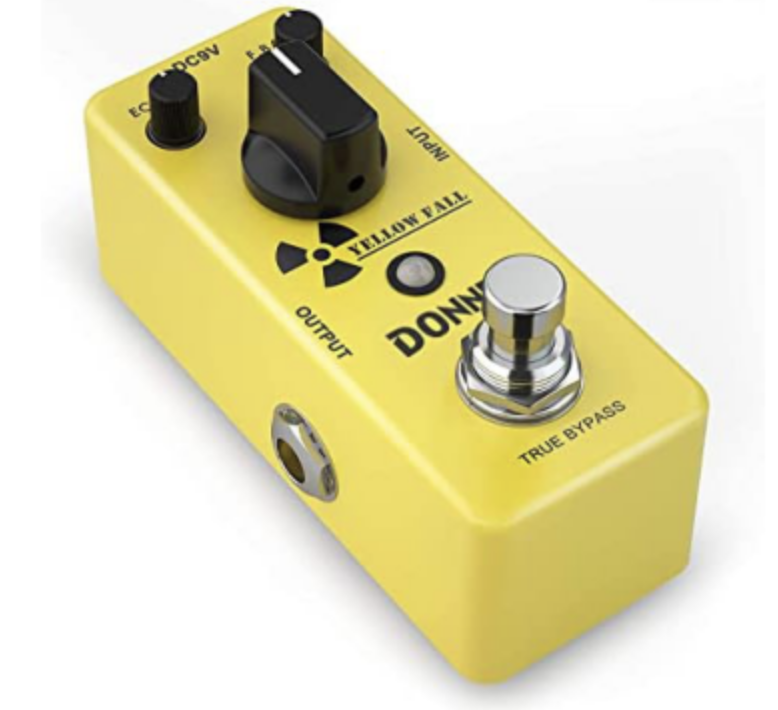
\includegraphics[width=.9\linewidth]{DSC210_Project_Report/images/recommendation3.png}
\end{minipage}
\label{fig:bpr_recommendations}
\end{figure}
We also look at the most similar items for a certain item using the cosine similarity of the item representations.

\subsection{SOTA Results}

Precision@10:

Recall@10:

\subsection{Compare and contrast}
\begin{itemize}
    \item
\end{itemize}


\section{Conclusion}
\begin{itemize}
    \item This project covered the problem of recommendation systems
    \item We implemented SVD as a way to extract latent feature represenations of users and items from the latent matrix factorization of the user-item interaction matrix.
    \item In the project, we used the Amazon-Reviews-2023 dataset.
    \item We used data science libraries with Python to develop our code on Google Colab and used GitHub for version control.
    \item Finally, we saw the shortcomings of the standard SVD, and explored two better solutions using Bayesian probabilistic model and Transformers.
\end{itemize}

\section{Acknowledgement}
We are grateful to Prof. Tsui-Wei Weng, Halıcıoğlu Data Science Institute, San Diego and the TAs for their continuous support, encouragement, and willingness to help us throughout this project.

\bibliographystyle{abbrv}
\bibliography{references}

\end{document}